\chapter{Diseño e Implementación} % Main chapter title

\label{Chapter3} % Change X to a consecutive number; for referencing this chapter elsewhere, use \ref{ChapterX}

\definecolor{mygreen}{rgb}{0,0.6,0}
\definecolor{mygray}{rgb}{0.5,0.5,0.5}
\definecolor{mymauve}{rgb}{0.58,0,0.82}

%%%%%%%%%%%%%%%%%%%%%%%%%%%%%%%%%%%%%%%%%%%%%%%%%%%%%%%%%%%%%%%%%%%%%%%%%%%%%
% parámetros para configurar el formato del código en los entornos lstlisting
%%%%%%%%%%%%%%%%%%%%%%%%%%%%%%%%%%%%%%%%%%%%%%%%%%%%%%%%%%%%%%%%%%%%%%%%%%%%%
\lstset{ %
  backgroundcolor=\color{white},   % choose the background color; you must add \usepackage{color} or \usepackage{xcolor}
  basicstyle=\footnotesize,        % the size of the fonts that are used for the code
  breakatwhitespace=false,         % sets if automatic breaks should only happen at whitespace
  breaklines=true,                 % sets automatic line breaking
  captionpos=b,                    % sets the caption-position to bottom
  commentstyle=\color{mygreen},    % comment style
  deletekeywords={...},            % if you want to delete keywords from the given language
  %escapeinside={\%*}{*)},          % if you want to add LaTeX within your code
  %extendedchars=true,              % lets you use non-ASCII characters; for 8-bits encodings only, does not work with UTF-8
  %frame=single,	                % adds a frame around the code
  keepspaces=true,                 % keeps spaces in text, useful for keeping indentation of code (possibly needs columns=flexible)
  keywordstyle=\color{blue},       % keyword style
  language=[ANSI]C,                % the language of the code
  %otherkeywords={*,...},           % if you want to add more keywords to the set
  numbers=left,                    % where to put the line-numbers; possible values are (none, left, right)
  numbersep=5pt,                   % how far the line-numbers are from the code
  numberstyle=\tiny\color{mygray}, % the style that is used for the line-numbers
  rulecolor=\color{black},         % if not set, the frame-color may be changed on line-breaks within not-black text (e.g. comments (green here))
  showspaces=false,                % show spaces everywhere adding particular underscores; it overrides 'showstringspaces'
  showstringspaces=false,          % underline spaces within strings only
  showtabs=false,                  % show tabs within strings adding particular underscores
  stepnumber=1,                    % the step between two line-numbers. If it's 1, each line will be numbered
  stringstyle=\color{mymauve},     % string literal style
  tabsize=2,	                   % sets default tabsize to 2 spaces
  title=\lstname,                  % show the filename of files included with \lstinputlisting; also try caption instead of title
  morecomment=[s]{/*}{*/}
}


%----------------------------------------------------------------------------------------
%	SECTION 1
%----------------------------------------------------------------------------------------
%\section{Análisis del software}
% 
%La idea de esta sección es resaltar los problemas encontrados, los criterios utilizados y la justificación de las decisiones que se hayan tomado.
%
%Se puede agregar código o pseudocódigo dentro de un entorno lstlisting con el siguiente código:
%
%\begin{verbatim}
%\begin{lstlisting}[caption= "un epígrafe descriptivo"]
%	las líneas de código irían aquí...
%\end{lstlisting}
%\end{verbatim}
%
%A modo de ejemplo:
%
%\begin{lstlisting}[label=cod:vControl,caption=Pseudocódigo del lazo principal de control.]  % Start your code-block
%
%#define MAX_SENSOR_NUMBER 3
%#define MAX_ALARM_NUMBER  6
%#define MAX_ACTUATOR_NUMBER 6
%
%uint32_t sensorValue[MAX_SENSOR_NUMBER];		
%FunctionalState alarmControl[MAX_ALARM_NUMBER];	//ENABLE or DISABLE
%state_t alarmState[MAX_ALARM_NUMBER];						//ON or OFF
%state_t actuatorState[MAX_ACTUATOR_NUMBER];			//ON or OFF
%
%void vControl() {
%
%	initGlobalVariables();
%	
%	period = 500 ms;
%		
%	while(1) {
%
%		ticks = xTaskGetTickCount();
%		
%		updateSensors();
%		
%		updateAlarms();
%		
%		controlActuators();
%		
%		vTaskDelayUntil(&ticks, period);
%	}
%}
%\end{lstlisting}

\section{Consideraciones generales}
\section{Generación automática}

	\begin{figure}[h]
	\centering
	%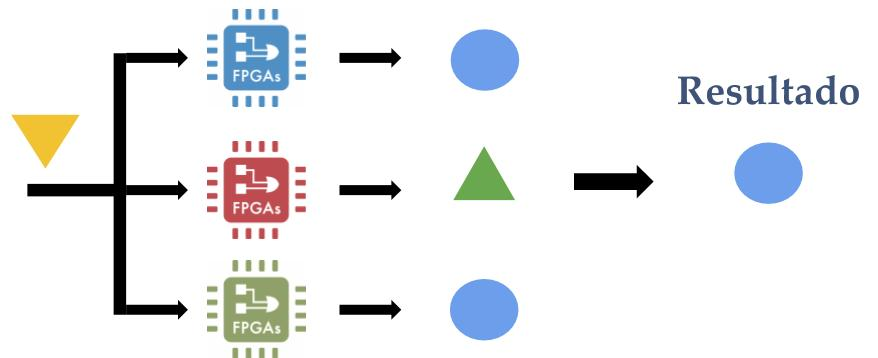
\includegraphics[scale=.3]{./Figures/Redundancia}
		\caption{HOLA}
		\label{fig:hola}
	\end{figure}
	\improvement{Incluir figura}	

\section{Módulo de nodos}

	\begin{figure}[h]
	\centering
	%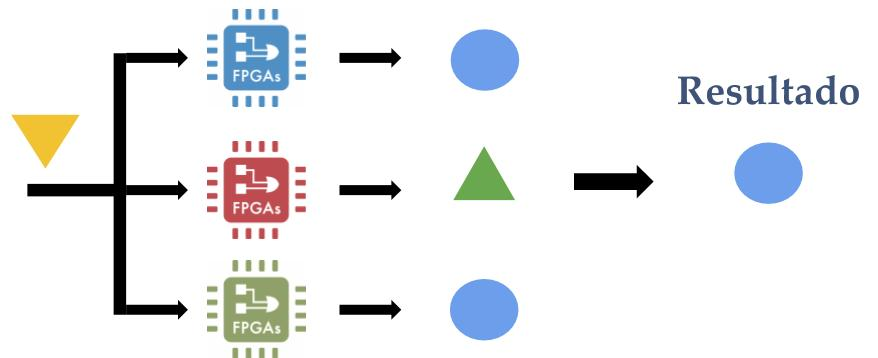
\includegraphics[scale=.3]{./Figures/Redundancia}
		\caption{HOLA}
		\label{fig:hola}
	\end{figure}
	\improvement{Incluir figura}	
	
\section{Módulo de cambios}

	\begin{figure}[h]
	\centering
	%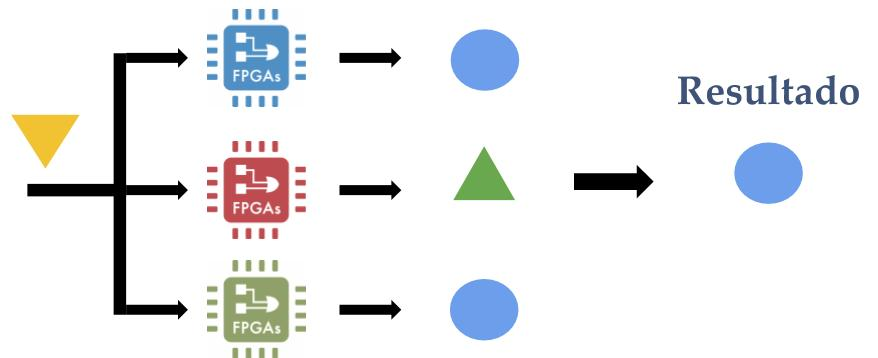
\includegraphics[scale=.3]{./Figures/Redundancia}
		\caption{HOLA}
		\label{fig:hola}
	\end{figure}
	\improvement{Incluir figura}	
	
\section{Módulo de red}

	\begin{figure}[h]
	\centering
	%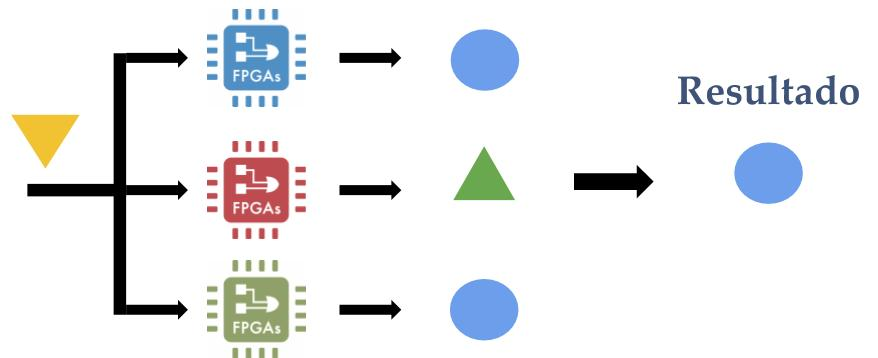
\includegraphics[scale=.3]{./Figures/Redundancia}
		\caption{HOLA}
		\label{fig:hola}
	\end{figure}
	\improvement{Incluir figura}	
	
\section{Módulos de adaptación a enclavamiento}

	\subsection{Módulo separador}
		\begin{figure}[h]
		\centering
		%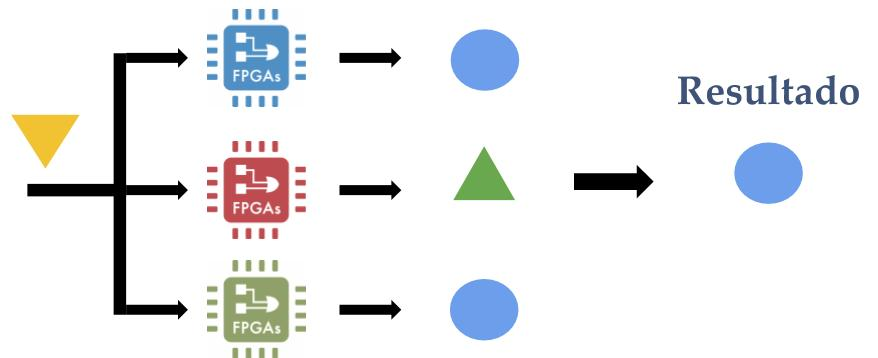
\includegraphics[scale=.3]{./Figures/Redundancia}
			\caption{HOLA}
			\label{fig:hola}
		\end{figure}
		\improvement{Incluir figura}
		
	\subsection{Módulo mediador}
		\begin{figure}[h]
		\centering
		%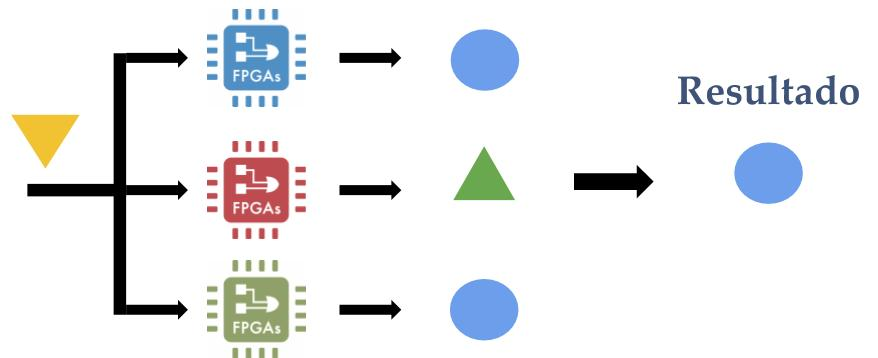
\includegraphics[scale=.3]{./Figures/Redundancia}
			\caption{HOLA}
			\label{fig:hola}
		\end{figure}
		\improvement{Incluir figura}		
	
\section{Módulos de procesamiento de tramas}

	\subsection{Módulo detector}
		\begin{figure}[h]
		\centering
		%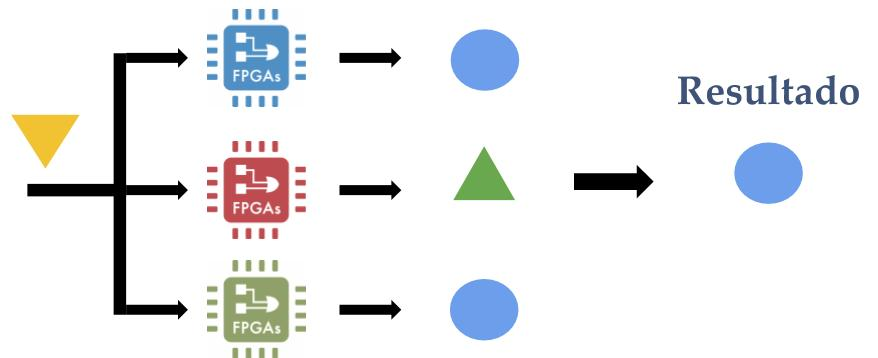
\includegraphics[scale=.3]{./Figures/Redundancia}
			\caption{HOLA}
			\label{fig:hola}
		\end{figure}
		\improvement{Incluir figura}	
	
	\subsection{Módulo registro}
		\begin{figure}[h]
		\centering
		%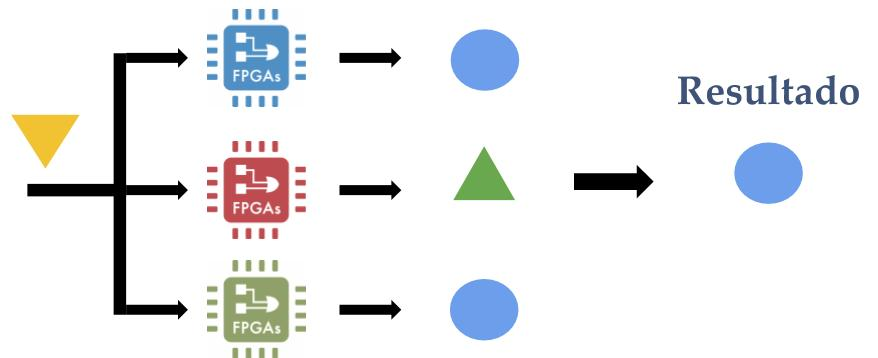
\includegraphics[scale=.3]{./Figures/Redundancia}
			\caption{HOLA}
			\label{fig:hola}
		\end{figure}
		\improvement{Incluir figura}
		
	\subsection{Módulo selector}
		\begin{figure}[h]
		\centering
		%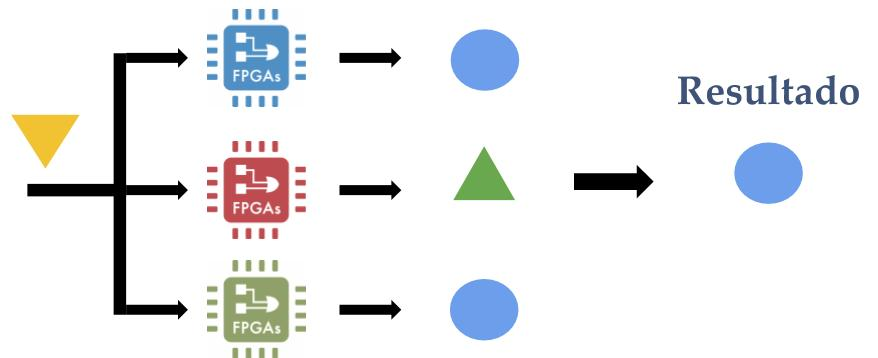
\includegraphics[scale=.3]{./Figures/Redundancia}
			\caption{HOLA}
			\label{fig:hola}
		\end{figure}
		\improvement{Incluir figura}	
		
\section{Módulo de comunicación UART}

		\begin{figure}[h]
		\centering
		%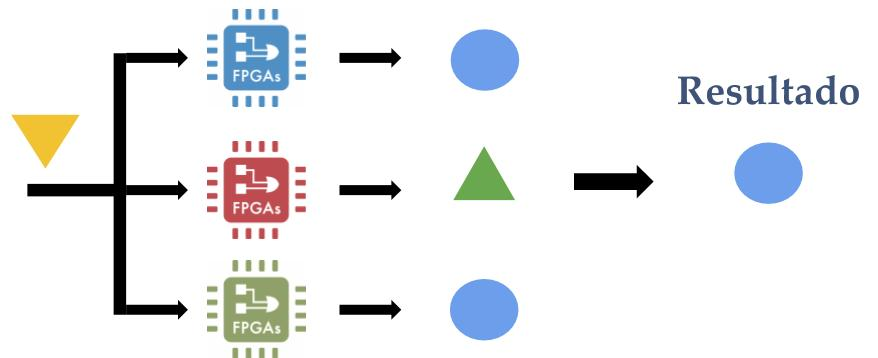
\includegraphics[scale=.3]{./Figures/Redundancia}
			\caption{HOLA}
			\label{fig:hola}
		\end{figure}
		\improvement{Incluir figura}

\section{Interfaz de comunicación Python}

		\begin{figure}[h]
		\centering
		%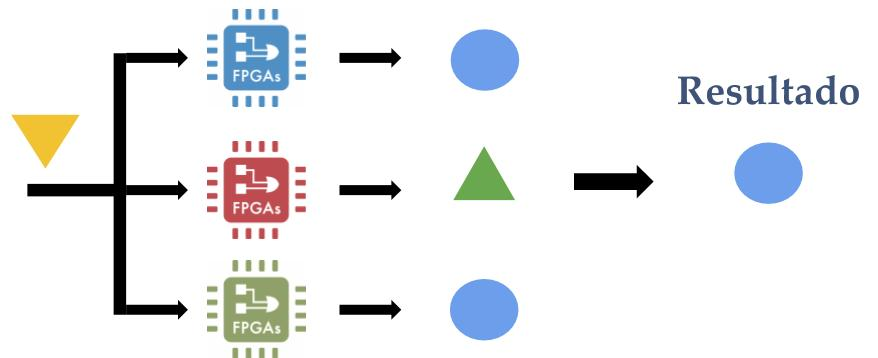
\includegraphics[scale=.3]{./Figures/Redundancia}
			\caption{HOLA}
			\label{fig:hola}
		\end{figure}
		\improvement{Incluir figura}